\chapter{Diseño e implementación} % Main chapter title

\label{Chapter3} % Change X to a consecutive number; for referencing this chapter elsewhere, use \ref{ChapterX}
En este capítulo se describe la arquitectura modular del sistema, diseñada para gestionar de forma independiente cada uno de sus componentes. La estructura implementada asegura flexibilidad durante el desarrollo, escalabilidad en su implementación y facilidad de mantenimiento a largo plazo.

\definecolor{mygreen}{rgb}{0,0.6,0}
\definecolor{mygray}{rgb}{0.5,0.5,0.5}
\definecolor{mymauve}{rgb}{0.58,0,0.82}

%%%%%%%%%%%%%%%%%%%%%%%%%%%%%%%%%%%%%%%%%%%%%%%%%%%%%%%%%%%%%%%%%%%%%%%%%%%%%
% parámetros para configurar el formato del código en los entornos lstlisting
%%%%%%%%%%%%%%%%%%%%%%%%%%%%%%%%%%%%%%%%%%%%%%%%%%%%%%%%%%%%%%%%%%%%%%%%%%%%%
\lstset{ %
  backgroundcolor=\color{white},   % choose the background color; you must add \usepackage{color} or \usepackage{xcolor}
  basicstyle=\footnotesize,        % the size of the fonts that are used for the code
  breakatwhitespace=false,         % sets if automatic breaks should only happen at whitespace
  breaklines=true,                 % sets automatic line breaking
  captionpos=b,                    % sets the caption-position to bottom
  commentstyle=\color{mygreen},    % comment style
  deletekeywords={...},            % if you want to delete keywords from the given language
  %escapeinside={\%*}{*)},          % if you want to add LaTeX within your code
  %extendedchars=true,              % lets you use non-ASCII characters; for 8-bits encodings only, does not work with UTF-8
  %frame=single,	                % adds a frame around the code
  keepspaces=true,                 % keeps spaces in text, useful for keeping indentation of code (possibly needs columns=flexible)
  keywordstyle=\color{blue},       % keyword style
  language=[ANSI]C,                % the language of the code
  %otherkeywords={*,...},           % if you want to add more keywords to the set
  numbers=left,                    % where to put the line-numbers; possible values are (none, left, right)
  numbersep=5pt,                   % how far the line-numbers are from the code
  numberstyle=\tiny\color{mygray}, % the style that is used for the line-numbers
  rulecolor=\color{black},         % if not set, the frame-color may be changed on line-breaks within not-black text (e.g. comments (green here))
  showspaces=false,                % show spaces everywhere adding particular underscores; it overrides 'showstringspaces'
  showstringspaces=false,          % underline spaces within strings only
  showtabs=false,                  % show tabs within strings adding particular underscores
  stepnumber=1,                    % the step between two line-numbers. If it's 1, each line will be numbered
  stringstyle=\color{mymauve},     % string literal style
  tabsize=2,	                   % sets default tabsize to 2 spaces
  title=\lstname,                  % show the filename of files included with \lstinputlisting; also try caption instead of title
  morecomment=[s]{/*}{*/}
}


%----------------------------------------------------------------------------------------
%	SECTION 1
%----------------------------------------------------------------------------------------
\section{Diseño general del sistema IoT}

El Sistema de Monitoreo de Calidad del Aire (SMCA) se basa en una arquitectura modular y desacoplada, organizada en cinco capas funcionale, \ref{fig:3_1-modular}. Esta estructura permite separar las responsabilidades de cada módulo, facilita el mantenimiento del software y habilita la evolución independiente de sus componentes. El diseño asegura que el backend funcione como el núcleo orquestador, gestionando tanto la ingesta de datos desde los nodos sensores como la entrega de información a la interfaz de usuario.

\vspace{0.5cm}
\begin{figure}[h]
    \centering
    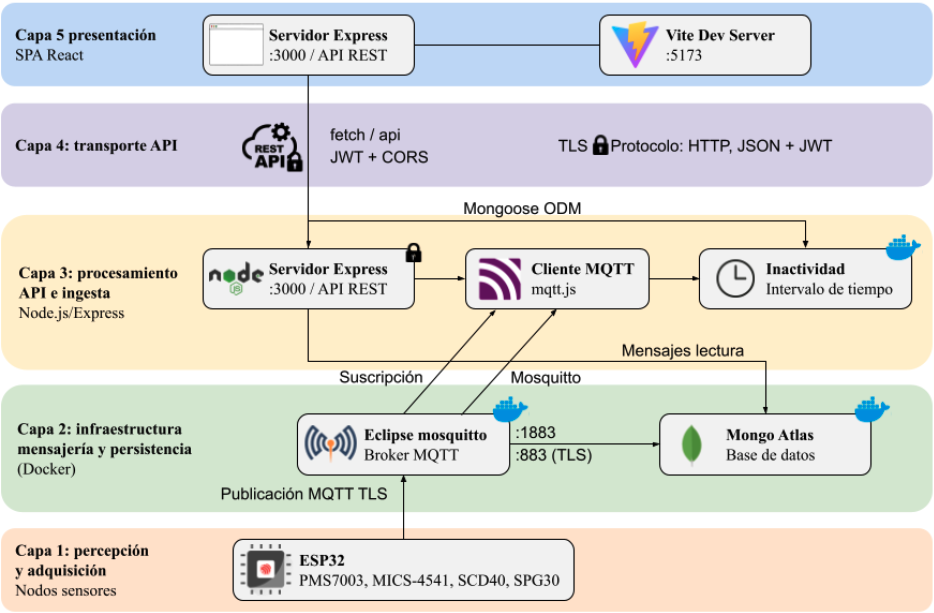
\includegraphics[width=1\linewidth]{Figures/3_1-Modular_Structure.png}
    \caption{Estructura modular del sistema organizada en capas independientes.}
    \label{fig:3_1-modular}
\end{figure}
\vspace{1cm}

La arquitectura se estructura en las siguientes capas:

\begin{itemize}
    \item Capa de percepción y adquisición: constituye el nivel físico del sistema y reside en los nodos sensores. El firmware, desarrollado para el microcontrolador ESP32 Heltec V3, gestiona la captura de variables ambientales mediante sensores específicos. Esta capa transforma las magnitudes físicas en tramas de datos digitales para su transmisión.
    
    \item Capa de transporte y mensajería: define los mecanismos de comunicación segura entre los nodos y el servidor. El sistema utiliza el protocolo MQTT sobre una conexión cifrada con TLS. Esta capa garantiza que el traslado de la información sea íntegro y que solo los dispositivos autorizados puedan publicar mensajes en el broker \texttt{Eclipse Mosquitto}.
    
    \item Capa de procesamiento e integración: funciona como el centro lógico de la solución y se implementa con Node.js. Este módulo actúa como un cliente que se suscribe a los tópicos de los sensores, valida la identidad de los dispositivos y calcula el índice de calidad del aire (AQI). Además, expone una interfaz de programación de aplicaciones (API) de tipo \texttt{REST} para el frontend.
    
    \item Capa de persistencia: gestiona el almacenamiento estructurado de la información mediante la base de datos MongoDB. El sistema emplea el mapeador de objetos \texttt{Mongoose} para organizar los documentos de lecturas, usuarios y dispositivos. Esta capa asegura que los datos históricos estén disponibles para consultas complejas y análisis temporales.
    
    \item Capa de presentación: representa la interfaz de interacción con el usuario final y se desarrolla con la biblioteca React. Este módulo consume los recursos de la API mediante peticiones HTTP y presenta las mediciones en un panel de control interactivo. La separación de esta capa permite que la visualización sea independiente de la lógica de captura de datos.
\end{itemize}

\section{Diseño e implementación del firmware (ESP32)}

El firmware constituye la lógica de control de los nodos sensores y se desarrolla sobre el entorno ESP-IDF v5.1.x. La implementación utiliza un enfoque modular mediante componentes independientes que interactúan bajo el sistema operativo de tiempo real \texttt{FreeRTOS}. Esta estructura permite la ejecución concurrente de tareas de adquisición, procesamiento y comunicación sin interferencias mutuas.

La organización general de estos módulos y su interacción con el hardware se detalla en la \ref{fig:3_2-modular}, que corresponde a 4 capas:
\begin{itemize}
    \item Capa de persistencia 
    \item Capa de drivers e infraestructura
    \item Capa de tareas
    \item Capa de entrada y gestores
\end{itemize}

\vspace{0.5cm}
\begin{figure}[h]
    \centering
    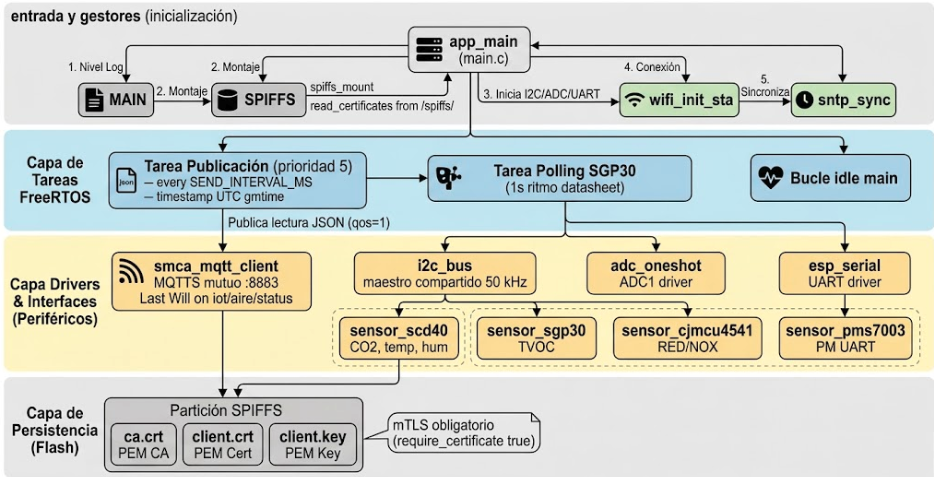
\includegraphics[width=1\linewidth]{Figures/3_2-Modular_Structure.png}
    \caption{Arquitectura del firmware.}
    \label{fig:3_2-modular}
\end{figure}

\subsection{Descripción del hardware: MCU y sensores}

La plataforma de hardware central es la placa Heltec WiFi LoRa 32 V3, basada en el microcontrolador ESP32-S3. Este dispositivo cuenta con un procesador de doble núcleo Xtensa LX7, 8 MB de memoria flash y 512 KB de \texttt{SRAM}. La selección de esta placa responde a su factor de forma compacto y la integración de periféricos necesarios para el monitoreo ambiental. En la tabla \ref{tab:3-sensores} se resumen los dispositivos integrados en el nodo y sus interfaces de comunicación.

\begin{table}[h]
    \centering
    \caption[Resumen de sensores utilizados]{Sensores seleccionados para el sistema SMCA.}
    \label{tab:3-sensores}
    \begin{tabular}{p{3.5cm} p{5.5cm} p{2.5cm}}
        \toprule
        \textbf{Sensor} & \textbf{Variable medida} & \textbf{Comunicación} \\
        \midrule
        PMS7003 & PM$_{2.5}$, PM$_{10}$ & UART  \\
        CJMCU-4541 & NO$_2$, CO, NH$_3$ & ADC \\
        SCD40 & CO$_2$, temperatura, humedad & I2C \\
        SGP30 & VOCs & I2C \\
        \bottomrule
    \end{tabular}
\end{table}

\subsection{Listado de conexiones y GPIOs utilizados}

El diseño electrónico asegura la integridad de las señales mediante una distribución de pines que evita conflictos en los buses de comunicación. El sistema utiliza un bus I2C maestro compartido para los sensores de Sensirion y canales del conversor analógico digital (ADC1) para el sensor de gases reductores.

En la tabla \ref{tab:conexiones-gpio} se detalla el mapeo físico implementado en el prototipo:

\begin{table}[h]
    \centering
    \caption{Listado de conexiones y asignación de GPIO.}
    \label{tab:conexiones-gpio}
    \begin{tabular}{p{3cm} p{3.5cm} p{3.5cm} p{3cm}}
        \toprule
        \textbf{Periférico} & \textbf{Interfaz} & \textbf{Pines GPIO} & \textbf{Notas técnicas} \\
        \midrule
        Bus I2C & Maestro compartido & SDA (41), SCL (42) & Pull-ups internos \\
        CJMCU-4541 & ADC1 & RED (4), NOX (6) & Atenuación 11dB \\
        PMS7003 & UART & TX (45), RX (46) & Trama 0x42 0x4D \\
        \bottomrule
    \end{tabular}
\end{table}

\subsection{Gestión de periféricos y controladores}

Cada sensor dispone de un controlador o driver específico dentro de la carpeta de componentes del proyecto. El firmware implementa una capa de abstracción que permite el uso de sensores reales o simuladores según la configuración del nodo.

\begin{itemize}
    \item Controlador I2C: gestiona el acceso al bus de forma \textit{thread-safe}, permitiendo que múltiples componentes soliciten lecturas sin colisiones.
    \item Controlador ADC: aplica una curva de ajuste (\textit{curve fitting}) para convertir los niveles de tensión del CJMCU-4541 en valores de concentración representativos.
    \item Controlador UART: gestiona la comunicación con el sensor de material particulado a través del puerto UART. Este componente utiliza un búfer de anillo (\textit{ring buffer}) para procesar las tramas digitales de forma asíncrona. Además, el controlador valida el \textit{checksum} de cada trama de 32 bytes antes de actualizar las variables globales del sistema, lo cual garantiza la integridad de los datos de PM$_{2.5}$ y PM$_{10}$.
    \item Manejo de errores: el sistema implementa reintentos con retardos específicos y reinicios de medición periódica tras detectar fallos consecutivos en el hardware.
\end{itemize}

La interconexión física entre el microcontrolador ESP32-S3 y los periféricos se detalla en la \ref{fig:3_3-conexiones-nodo}.

\vspace{0.5cm}
\begin{figure}[h]
    \centering
    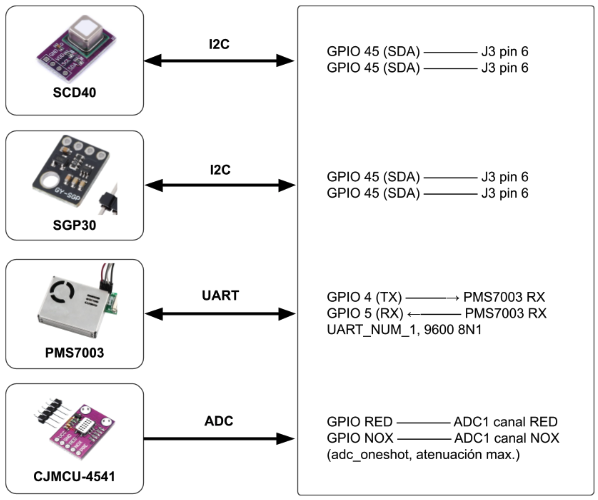
\includegraphics[width=0.9\linewidth]{Figures/3_3-diagrama_sensores.png}
    \caption{Diagrama de conexiones del nodo.}
    \label{fig:3_3-conexiones-nodo}
\end{figure}

\subsection{Seguridad y almacenamiento en SPIFFS}

Para garantizar la seguridad en el transporte de datos, el nodo utiliza una partición \texttt{SPIFFS} (del inglés, Serial Peripheral Interface Flash File System). En este sistema de archivos se almacenan los certificados de la autoridad certificadora (\texttt{ca.crt}), el certificado del cliente (\texttt{client.crt}) y la clave privada (\texttt{client.key}).

Esta arquitectura permite implementar la autenticación mutua (\texttt{mTLS}), donde las credenciales se cargan en la memoria \texttt{RAM} únicamente durante el proceso de apretón de manos con el servidor, separando la identidad del dispositivo de la lógica de programación.

\subsection{Flujo de publicación y mensajería MQTT}

El intercambio de información con el backend se basa en el protocolo \texttt{MQTT} sobre el puerto 8883. La tarea de publicación se ejecuta con prioridad 5 y realiza las siguientes acciones:

\begin{itemize}
    \item Recolecta las últimas mediciones disponibles de los controladores.
    \item Construye un objeto \texttt{JSON} que incluye el identificador del nodo y la marca de tiempo ISO 8601.
    \item Envía el mensaje con calidad de servicio \texttt{QoS 1}, asegurando al menos una entrega exitosa.
    \item Gestiona el mensaje de última voluntad (\textit{Last Will}) para notificar desconexiones inesperadas.
\end{itemize}

\subsection{Flujo de ejecución}

El firmware sigue un ciclo de vida diseñado para priorizar la disponibilidad de los recursos críticos. La lógica de arranque se describe en la

El proceso se divide en:

\begin{itemize}
    \item Inicialización: ajuste de logs, montaje de \texttt{SPIFFS} y arranque de controladores físicos.
    \item Conectividad: establecimiento de Wi-Fi y sincronización horaria mediante \texttt{SNTP}.
    \item Arranque de servicios: inicio del cliente MQTT y creación de las tareas de \texttt{FreeRTOS}.
\end{itemize}

\subsection{Configuración multi-nodo}

La arquitectura permite el despliegue de múltiples nodos mediante una configuración centralizada en el archivo \texttt{config.h}. Este diseño facilita la escalabilidad del sistema, ya que cada nodo puede ser personalizado (activando o desactivando sensores específicos) y configurado con su propio par de claves criptográficas sin alterar el binario principal del firmware.

\section{Diseño e implementación del backend}

El backend del sistema SMCA funciona como un motor de convergencia que integra la recepción de telemetría IoT, la persistencia en base de datos y la exposición de una interfaz de programación de aplicaciones (API). Se desarrolla sobre el entorno de ejecución Node.js, utilizando un modelo de arquitectura monolítica modular donde el servidor gestiona simultáneamente las conexiones HTTP y la suscripción al broker MQTT.

\subsection{Stack tecnológico y dependencias}

La selección de tecnologías prioriza la escalabilidad asíncrona y la facilidad de integración con formatos de datos JSON. En la tabla \ref{tab:stack-backend} se detallan las bibliotecas fundamentales que conforman el núcleo del servidor.

\begin{table}[h]
    \centering
    \caption[Stack tecnológico del backend]{Componentes del desarrollo del servidor.}
    \label{tab:stack-backend}
    \begin{tabular}{p{2.8cm} p{1.5cm} p{8cm}}
        \toprule
        \textbf{Paquete} & \textbf{Versión} & \textbf{Rol en el sistema} \\
        \midrule
        \texttt{Express} & \texttt{4.18} & Framework para la creación de la \texttt{API REST}. \\
        \texttt{Mongoose} & \texttt{7.5} & \texttt{ODM} para la comunicación con MongoDB. \\
        \texttt{mqtt} & \texttt{5.3} & Cliente para la suscripción al broker y recepción de datos. \\
        \texttt{jsonwebtoken} & \texttt{9.0} & Gestión de seguridad mediante tokens JWT. \\
        \texttt{bcrypt} & \texttt{6.0} & Algoritmo de cifrado para contraseñas de usuarios. \\
        \bottomrule
    \end{tabular}
\end{table}

\subsection{Estructura de componentes y organización del proyecto}

Para facilitar el mantenimiento y la extensibilidad del código, el proyecto sigue una estructura de directorios basada en la separación de responsabilidades. Cada entidad del sistema (dispositivos, lecturas, usuarios) cuenta con su propio modelo, controlador y rutas.

La organización jerárquica del código en el directorio \texttt{src/} se describe a continuación:

\begin{itemize}
    \item \textbf{\texttt{db/}}: contiene la lógica de conexión y la definición de los esquemas de \texttt{Mongoose} (Modelos).
    \item \textbf{\texttt{controllers/}}: implementa la lógica de negocio y procesa las peticiones de entrada.
    \item \textbf{\texttt{routes/}}: define los \textit{endpoints} de la API y asocia los métodos HTTP con sus controladores.
    \item \textbf{\texttt{middleware/}}: aloja las funciones de interceptación, principalmente para la validación de sesiones y roles de usuario.
    \item \textbf{\texttt{utils/}}: funciones auxiliares, incluyendo el calculador de AQI y el emisor de eventos SSE.
\end{itemize}

\subsection{Arquitectura de procesamiento y lógica IoT}

El backend opera como un proceso único que combina tres flujos de trabajo paralelos dentro del \textit{event loop} de Node.js:

\begin{itemize}
    \item Recepción IoT (cliente MQTT): el servidor se conecta al broker \texttt{Mosquitto} mediante el archivo \texttt{mqttClient.js}. Al recibir un mensaje en el tópico de lectura, valida la autenticidad del dispositivo y normaliza los datos.
    \item Cálculo del AQI: antes de la persistencia, el sistema utiliza el componente \texttt{aqiCalculator.js}. Este módulo implementa las fórmulas de la EPA (\textit{Environmental Protection Agency}) para transformar concentraciones de PM$_{2.5}$, CO2 y CO$_{2}$ en un índice de calidad de aire adimensional, facilitando la interpretación para el usuario final.
    \item Persistencia y Eventos: una vez procesada, la lectura se almacena en MongoDB Atlas. Simultáneamente, el backend utiliza un \texttt{EventEmitter} para disparar una notificación hacia el canal SSE, logrando que los clientes web actualicen sus gráficos instantáneamente sin recargar la página.
\end{itemize}

\subsection{Seguridad y control de Acceso}

La protección de la API se basa en un esquema de autenticación por \textit{tokens}. El flujo de seguridad implementado garantiza que las acciones críticas (como registrar un nuevo nodo o crear una zona) estén restringidas:

\begin{itemize}
    \item Autenticación: al iniciar sesión, el servidor genera un \texttt{JWT} firmado que expira tras un periodo determinado.
    \item Autorización: los \textit{middlewares} \texttt{authMiddleware} y \texttt{requireRole} verifican el rango del usuario en cada petición. El sistema soporta roles de admin (control total) y viewer (solo lectura de datos ambientales).
    \item Cifrado: las contraseñas nunca se almacenan en texto plano; se utiliza la biblioteca \texttt{bcrypt} con un factor de costo (\textit{salt}) adecuado para mitigar ataques de fuerza bruta.
\end{itemize}

\subsection{Interfaz de Programación de Aplicaciones (API REST)}

La \texttt{API} permite la interacción del frontend con el ecosistema de datos. Se han definido rutas específicas para la gestión administrativa y la visualización de datos históricos.

\begin{table}[h]
    \centering
    \caption[Resumen de rutas principales de la API]{Endpoints para la gestión y consulta de telemetría.}
    \label{tab:rutas-api}
    \begin{tabular}{p{4cm} p{2cm} p{6cm}}
        \toprule
        \textbf{Ruta} & \textbf{Método} & \textbf{Propósito} \\
        \midrule
        \texttt{/api/auth} & \texttt{POST} & Autenticación de usuarios y generación de \texttt{JWT}. \\
        \texttt{/api/lecturas} & \texttt{GET} & Consulta de históricos con filtros de fecha y zona. \\
        \texttt{/api/sse} & \texttt{GET} & Canal abierto para recepción de datos en tiempo real. \\
        \texttt{/api/dispositivos} & \texttt{POST} & Registro y vinculación de nuevos nodos sensores. \\
        \bottomrule
    \end{tabular}
\end{table}

\section{Diseño e implementación del frontend}

El frontend del sistema SMCA es una aplicación de página única (\textit{Single Page Application} o SPA) desarrollada con la librería React. Su objetivo principal es ofrecer un tablero de control (\textit{dashboard}) intuitivo que permita la visualización de datos en tiempo real, el análisis de históricos y la gestión administrativa del ecosistema IoT.

\subsection{Stack tecnológico y herramientas de desarrollo}

La selección de tecnologías se enfoca en la modularidad y el rendimiento en la renderización de gráficos complejos. En la tabla \ref{tab:stack-frontend} se detallan las bibliotecas núcleo del cliente web.

\begin{table}[h]
    \centering
    \caption[Stack tecnológico del frontend]{Bibliotecas y herramientas utilizadas en el desarrollo de la interfaz de usuario.}
    \label{tab:stack-frontend}
    \begin{tabular}{p{3.5cm} p{2cm} p{6.5cm}}
        \toprule
        \textbf{Paquete} & \textbf{Versión} & \textbf{Rol en el sistema} \\
        \midrule
        React & \texttt{18.2} & Librería base para la creación de componentes de interfaz. \\
        Vite & \texttt{5.0} & Herramienta de construcción (\textit{bundler}) y servidor de desarrollo. \\
        \texttt{Recharts} & \texttt{3.7} & Generación de gráficos interactivos de series temporales. \\
        Materialize & \texttt{1.0} & Framework de diseño basado en \textit{Material Design} de Google. \\
        Luxon & \texttt{3.5} & Gestión avanzada de fechas y zonas horarias. \\
        \bottomrule
    \end{tabular}
\end{table}

\subsection{Arquitectura basada en componentes y carpetas}

La aplicación sigue una estructura organizada por responsabilidades, lo que facilita la reutilización de código y el escalado de la plataforma. La organización jerárquica en el directorio \texttt{src/} es la siguiente:

\begin{itemize}
    \item \texttt{context/}: implementa la gestión de estado global mediante la \textit{Context API} de React. Incluye el \texttt{AuthContext} para la sesión del usuario y el \texttt{ThemeContext} para el soporte de modo claro y oscuro.
    \item \texttt{layout/}: define la estructura visual común, como la barra de navegación (\texttt{Navbar}) y el menú lateral (\texttt{Sidenav}), el cual se filtra dinámicamente según el rol del usuario.
    \item \texttt{views/}: contiene las páginas principales de la aplicación (Inicio, Histórico, Dispositivos, Zonas, Usuarios).
    \item \texttt{components/}: aloja elementos de interfaz reutilizables, como ventanas modales de edición y la escala de referencia del AQI.
\end{itemize}

\subsection{Gestión de datos: REST y Server-Sent Events (SSE)}

El frontend se comunica con el backend mediante dos mecanismos complementarios que aseguran la disponibilidad de los datos:

\begin{itemize}
    \item Consumo de API REST: Para operaciones \textit{CRUD} (Crear, Leer, Actualizar, Borrar) y consultas de datos históricos, se utiliza la API \texttt{fetch} nativa. Todas las peticiones incluyen el \textit{token} \texttt{JWT} en las cabeceras de autorización.
    \item Visualización en Tiempo Real (SSE): En la vista de históricos y el dashboard principal, se utiliza la interfaz \texttt{EventSource}. Esta conexión persistente permite recibir actualizaciones de sensores instantáneamente desde el backend, logrando que los gráficos de \texttt{Recharts} se actualicen automáticamente sin intervención del usuario.
\end{itemize}

\subsection{Diseño de experiencia de usuario (UX) y seguridad}

La interfaz ha sido diseñada bajo criterios de accesibilidad y seguridad:

\begin{itemize}
    \item Control de acceso (Guards): El componente \texttt{RequireAuth} protege las rutas privadas. Si un usuario intenta acceder a una vista administrativa sin los permisos adecuados (rol \texttt{admin}), el sistema lo redirige automáticamente o deniega el acceso.
    \item Diseño responsivo: Gracias al sistema de \textit{grids} de \texttt{Materialize CSS}, la plataforma es totalmente funcional tanto en monitores de escritorio como en dispositivos móviles.
    \item Visualización crítica: Se utiliza una lógica de colores normalizada (basada en el estándar de la EPA) para que el usuario identifique visualmente el estado de la calidad del aire (ej. Verde para "Bueno", Rojo para "Insalubre").
\end{itemize}

\subsection{Flujo de compilación para producción}

A diferencia del backend, el frontend se distribuye como código estático. El proceso consiste en:

Ejecutar \texttt{npm run build} para que Vite genere una versión optimizada y minificada en la carpeta \texttt{dist/}.

\begin{itemize}
    \item Sincronizar estos archivos con el bucket de \texttt{Amazon S3}.
    \item Invalidar la caché en \texttt{Amazon CloudFront} para que los usuarios finales reciban la versión más reciente de la interfaz.
\end{itemize}


\section{Diseño de la base de datos}

El sistema utiliza MongoDB como motor de base de datos documental. La elección de una solución \texttt{NoSQL} responde a los requisitos propios de una plataforma IoT: alta frecuencia de escrituras, parámetros ambientales variables por dispositivo y la necesidad de escalar horizontalmente sin interrupciones por migraciones de esquema.

En la tabla \ref{tab:tecnologias-db} se detallan los componentes principales del stack de persistencia.

\begin{table}[h]
    \centering
    \caption[Componentes de la base de datos]{Tecnologías y servicios utilizados para la persistencia de datos en el sistema SMCA.}
    \label{tab:tecnologias-db}
    \begin{tabular}{p{4.5cm} p{7.5cm}}
        \toprule
        \textbf{Componente} & \textbf{Detalle} \\
        \midrule
        Motor & MongoDB 6 \\
        \texttt{ODM} & \texttt{Mongoose} 7 (Node.js) \\
        Servicio en producción & MongoDB Atlas (Cloud) \\
        Entorno de desarrollo & Docker (\texttt{image: mongo:6}) \\
        \bottomrule
    \end{tabular}
\end{table}

\subsection{Modelo de datos y colecciones}

A diferencia de las bases de datos relacionales, MongoDB organiza la información en colecciones de documentos JSON. Para el sistema SMCA, se ha diseñado un esquema que prioriza la velocidad de consulta del panel de control y la trazabilidad de las mediciones, ver \ref{fig:3_4-diagrama-e-r}.

\vspace{0.5cm}
\begin{figure}[h]
    \centering
    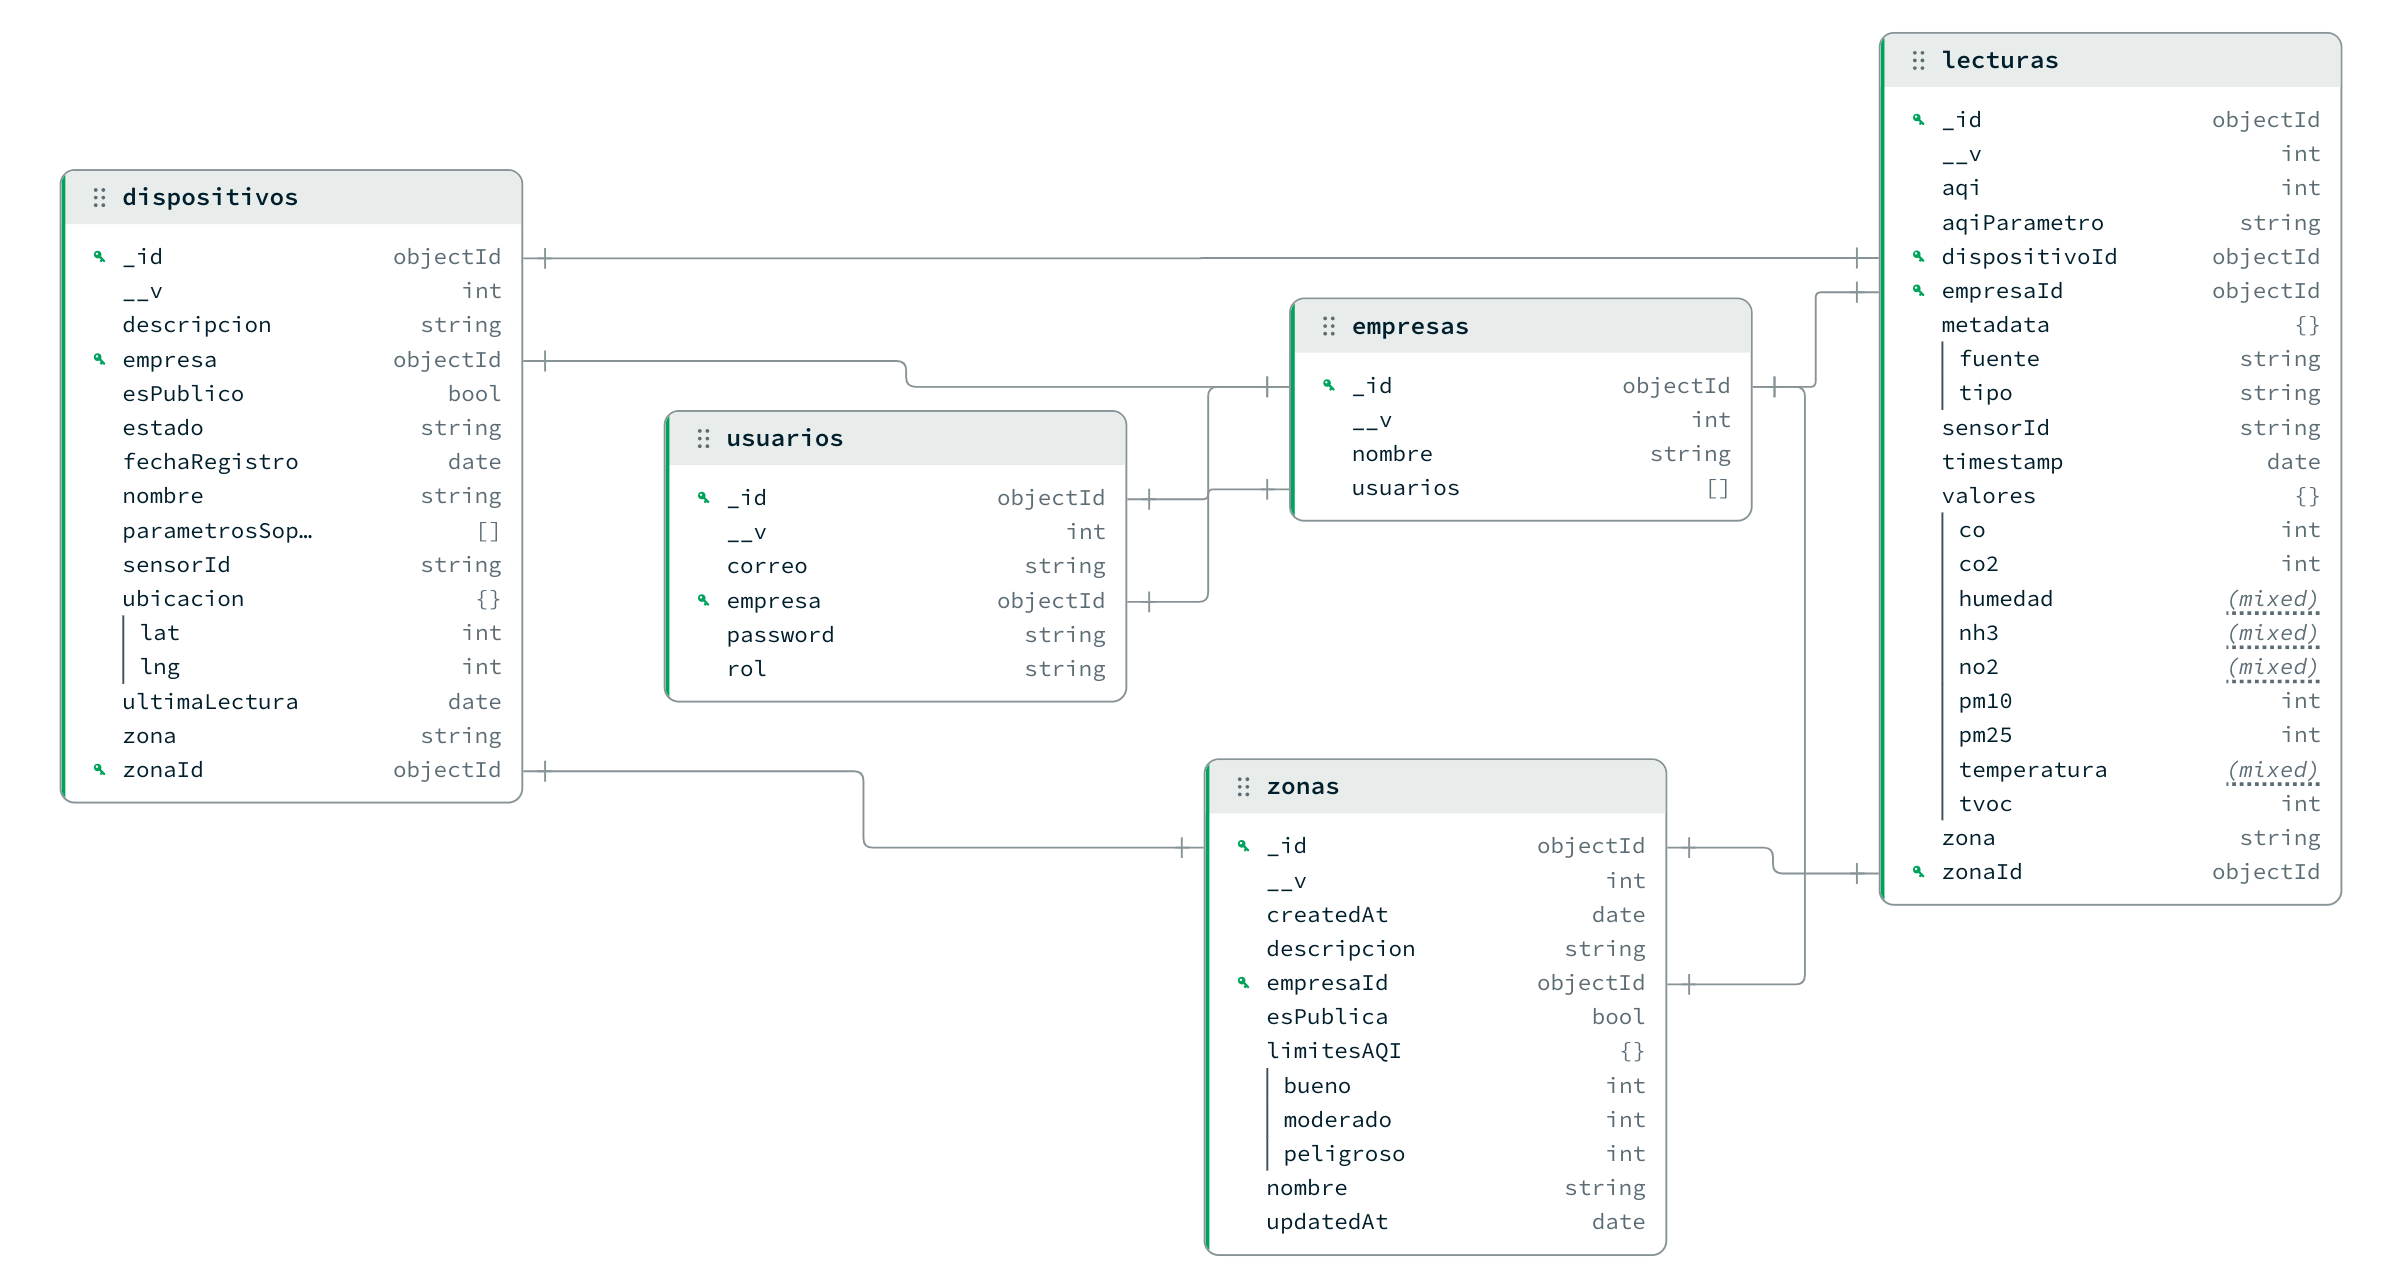
\includegraphics[width=1\linewidth]{Figures/3_4-diagrama_entidad-relacion.png}
    \caption{Diagrama entidad relación.}
    \label{fig:3_4-diagrama-e-r}
\end{figure}

Las principales colecciones implementadas son las siguientes:

\begin{itemize}
    \item Empresas: actúa como el nodo raíz para el soporte multi-entidad (\textit{multi-tenant}), permitiendo el aislamiento de datos entre diferentes organizaciones.
    \item Dispositivos: almacena la configuración técnica de los nodos, incluyendo el identificador único (\texttt{chipId}), el estado de los sensores y la relación con la zona asignada.
    \item Lecturas: es la colección con mayor volumen de datos. Cada documento registra las variables de calidad del aire, el AQI calculado y la marca de tiempo (\texttt{timestamp}) generada por el nodo sensor.
    \item Usuarios: gestiona las credenciales cifradas y los roles de acceso (admin o viewer) mediante el esquema de seguridad del sistema.
\end{itemize}

\subsection{Estrategia de indexación y rendimiento}

Dada la naturaleza temporal de los datos de calidad del aire, el rendimiento de las consultas depende de una indexación eficiente. El sistema implementa índices compuestos en la colección de lecturas, asociando el \texttt{dispositivo\textunderscore id} con el \texttt{timestamp}. Esta configuración optimiza la recuperación de series históricas necesarias para los gráficos de tendencias en el frontend.

Además, se ha configurado un índice de expiración (\texttt{TTL Index}) opcional para la purga automática de datos antiguos, lo cual permite gestionar el crecimiento del almacenamiento en el tier gratuito de \texttt{MongoDB Atlas}.

\subsection{Integración con el backend mediante Mongoose}

La interacción entre el servidor Node.js y la base de datos se realiza a través de \texttt{Mongoose}. Este \texttt{ODM} (del inglés, Object Document Mapper) permite definir esquemas con validación de tipos de datos en el lado de la aplicación.

El proceso de persistencia sigue un flujo de validación estricto:

\begin{itemize}
    \item El backend recibe la telemetría vía MQTT.
    \item Se instancia un modelo de \texttt{Mongoose} que verifica la integridad de los campos obligatorios.
    \item Se realiza la inserción asíncrona en la colección correspondiente, gestionando posibles errores de conexión mediante una política de reintentos definida en el controlador de base de datos.
\end{itemize}

\section{Comunicación IoT}

La comunicación entre los nodos sensores y el servidor central constituye el eje crítico del sistema. Para asegurar una transferencia de datos eficiente en entornos de red variables y garantizar la confidencialidad de la información ambiental, el sistema implementa el protocolo MQTT sobre una capa de transporte seguro TLS.

\subsection{Protocolo de mensajería: MQTT}

Se seleccionó \texttt{MQTT} v3.1.1 debido a su arquitectura basada en el modelo de publicación y suscripción (\textit{pub/sub}). El flujo de información se organiza mediante tópicos específicos que definen el canal y el propósito de cada mensaje, como se detalla en la tabla \ref{tab:topicos-mqtt}.

\begin{table}[h]
    \centering
    \caption[Definición de tópicos MQTT]{Tópicos utilizados para la telemetría y el control de estado de los nodos.}
    \label{tab:topicos-mqtt}
    \begin{tabular}{p{3.5cm} p{2.5cm} p{1cm} p{1cm} p{3.5cm}}
        \toprule
        \textbf{Tópico} & \textbf{Dirección} & \textbf{QoS} & \textbf{Ret.} & \textbf{Descripción} \\
        \midrule
        \texttt{iot/aire/lectura} & Nodo $\rightarrow$ Broker & 1 & \texttt{false} & Publicación de telemetría. \\
        \texttt{iot/aire/status} & Broker $\rightarrow$ Subs. & 1 & \texttt{true} & Estado de conexión (\textit{Last Will}). \\
        \bottomrule
    \end{tabular}
\end{table}

Al establecer la conexión, el cliente registra un mensaje de última voluntad (\textit{Last Will and Testament}) en el broker. Si el nodo pierde la conexión de forma inesperada, el servidor publica automáticamente un \texttt{JSON} en el tópico \texttt{iot/aire/status} con el identificador del dispositivo y el estado \texttt{offline}. Al utilizar el flag de retención (\textit{retain}), cualquier suscriptor nuevo, como el backend, recibe inmediatamente el último estado conocido del nodo.

\subsection{Seguridad mediante TLS y autenticación mutua}

Dada la exposición de los nodos a redes públicas, la seguridad se implementa mediante MQTTS (puerto 8883), utilizando el protocolo TLS v1.2. El sistema eleva el estándar de seguridad mediante Autenticación Mutua (mTLS), requiriendo un intercambio bidireccional de certificados:

\begin{itemize}
    \item Validación del servidor: el nodo verifica la identidad del broker utilizando el certificado de la Autoridad Certificadora (\texttt{ca.crt}) almacenado en \texttt{SPIFFS}.
    \item Validación del cliente: el broker exige al nodo presentar su certificado (\texttt{client.crt}) y demuestra la posesión de su clave privada (\texttt{client.key}) durante el apretón de manos (\textit{handshake}).
\end{itemize}

\subsection{Estructura del payload JSON y marcas de tiempo}

La información ambiental se transporta en formato JSON. El diseño del \textit{payload} es dinámico para optimizar el uso del ancho de banda y la memoria del microcontrolador (buffer limitado a 460 bytes). Los campos como \texttt{co2}, \texttt{temp} y \texttt{hum} se incluyen únicamente si el sensor \texttt{SCD40} entrega una lectura válida (\texttt{data\textunderscore ready = 1}); de lo contrario, se omiten para evitar el envío de datos nulos o erróneos.

Un ejemplo de la trama generada por el componente \texttt{sensor\textunderscore sim.c} es el siguiente:

\begin{verbatim}
    {
    "sensorId": "esp32-air-001",
    "timestamp": "2026-04-02T20:09:29Z",
    "pm25": 14.00, "pm10": 16.00,
    "co2": 450.0, "tvoc": 120,
    "temp": 23.5, "hum": 74.0
    }
\end{verbatim}

La marca de tiempo se genera con la función \texttt{gmtime()} sobre el tiempo de sistema sincronizado vía \texttt{SNTP}. Se utiliza exclusivamente el estándar \texttt{UTC} con formato ISO 8601 (\texttt{YYYY-MM-DDTHH:MM:SSZ}), lo cual garantiza que la persistencia en la base de datos sea independiente de la ubicación geográfica del nodo o del servidor.

\section{Despliegue del sistema en la nube}

El despliegue del sistema SMCA adopta una arquitectura híbrida que combina servicios de computación en la nube (\textit{cloud}) con el alojamiento de contenedores en servidores virtuales. Esta estrategia permite un balance óptimo entre escalabilidad, seguridad y costos operativos. El sistema opera en dos entornos diferenciados: un entorno de desarrollo basado en Docker local y un entorno de producción distribuido.

En la tabla \ref{tab:entornos-despliegue} se comparan las tecnologías utilizadas en ambos escenarios.

\begin{table}[h]
    \centering
    \caption[Comparativa de entornos de despliegue]{Diferencias entre entorno local y producción.}
    \label{tab:entornos-despliegue}
    \begin{tabular}{p{3.5cm} p{4cm} p{4.5cm}}
        \toprule
        \textbf{Componente} & \textbf{Entorno Local} & \textbf{Producción (AWS/Cloud)} \\
        \midrule
        Frontend & Vite dev server & S3 + CloudFront (CDN) \\
        Backend & Docker (Node.js) & Docker en EC2 \\
        Broker MQTT & \texttt{Mosquitto} local & \texttt{Mosquitto} en EC2 \\
        Base de datos & MongoDB local & MongoDB Atlas (Cloud) \\
        Seguridad TLS & TLS / PKI propia & Let's Encrypt + mTLS \\
        \bottomrule
    \end{tabular}
\end{table}

\subsection{Arquitectura de producción y red}

La infraestructura se apoya en los servicios de \texttt{AWS} para garantizar la alta disponibilidad de la interfaz y una gestión eficiente de la telemetría. En la tabla \ref{tab:servidores-servicios} se detallan las responsabilidades de cada componente.

\begin{table}[h]
    \centering
    \caption[Componentes de infraestructura y servicios]{Servicios y herramientas que conforman la arquitectura de producción del SMCA.}
    \label{tab:servidores-servicios}
    \begin{tabular}{p{3.5cm} p{3.5cm} p{5.5cm}}
        \toprule
        \textbf{Componente} & \textbf{Servicio} & \textbf{Responsabilidad} \\
        \midrule
        \texttt{EC2} & AWS & Ejecuta \texttt{Docker Compose} con el backend y \texttt{Mosquitto}. \\
        \texttt{S3} & AWS & Aloja los archivos estáticos del frontend compilado. \\
        \texttt{CloudFront} & AWS & \texttt{CDN} y terminación TLS para el frontend. \\
        MongoDB Atlas & MongoDB & Base de datos gestionada externa a la instancia \texttt{EC2}. \\
        Caddy & Software & \texttt{Reverse proxy} con TLS automático para el backend. \\
        Hostinger & DNS & Gestión de dominios y resolución de registros. \\
        \bottomrule
    \end{tabular}
\end{table}

El flujo de tráfico se organiza mediante los siguientes puntos de presencia:
\begin{itemize}
    \item Entrega de contenido (CDN): el frontend estático reside en un bucket de \texttt{Amazon S3} y se distribuye globalmente a través de \texttt{CloudFront}. Esta configuración asegura tiempos de carga mínimos y reduce la latencia para el usuario final.
    \item Servidor de aplicaciones (EC2): una instancia de computación \texttt{Amazon EC2} aloja los contenedores Docker del backend y del broker MQTT.
    \item Proxy Inverso: el servidor Caddy actúa como punto de entrada único para el tráfico HTTPS. Este componente gestiona automáticamente la renovación de certificados de \textit{Let's Encrypt} y redirige las peticiones hacia el contenedor del backend.
\end{itemize}

\subsection{DNS y gestión de dominios}

El sistema utiliza Hostinger como gestor de DNS externo. Se han definido dos dominios principales para separar el tráfico de usuario de la comunicación de los nodos sensores, tal como se detalla en la tabla \ref{tab:dns-dominios}.

\begin{table}[h]
    \centering
    \caption[Configuración de registros DNS]{Asignación de dominios y servicios finales.}
    \label{tab:dns-dominios}
    \begin{tabular}{p{4.5cm} p{2cm} p{5.5cm}}
        \toprule
        \textbf{Dominio} & \textbf{Registro} & \textbf{Servicio final} \\
        \midrule
        \texttt{air.mydatavibe.com} & \texttt{CNAME} & \texttt{CloudFront} $\rightarrow$ \texttt{S3} (Frontend) \\
        \texttt{smca.mydatavibe.com} & \texttt{A} & \texttt{IP} Elástica \texttt{EC2} $\rightarrow$ \texttt{Caddy} $\rightarrow$ Backend \\
        \bottomrule
    \end{tabular}
\end{table}

\subsection{Estrategia de contenedores y orquestación}

Para asegurar la paridad entre entornos, el sistema utiliza Docker y \texttt{Docker Compose}. La red interna \texttt{smca\textunderscore net} permite que los servicios se comuniquen mediante sus nombres de contenedor como resolución DNS interna. En producción, la configuración se divide en dos módulos críticos ejecutados en \texttt{EC2}:

\begin{itemize}
    \item \textbf{Imagen Mosquitto}: basada en \texttt{eclipse-mosquitto:2.0}, gestiona la comunicación MQTTS en el puerto 8883. Utiliza montajes de volumen persistentes para registros (\texttt{log}) y datos, además de montajes de solo lectura para la PKI y las ACL.
    \item \textbf{Imagen Backend}: construida sobre Node.js 18, procesa la telemetría y expone la \texttt{API} en el puerto 3000, el cual es redirigido por el servidor Caddy hacia el puerto 443 externo.
\end{itemize}

El frontend se excluye de la orquestación en producción; los archivos resultantes de la compilación (\texttt{dist/}) se sincronizan directamente con \texttt{S3} y la caché de \texttt{CloudFront} se invalida para reflejar los cambios.

\subsection{Capas de seguridad en el despliegue}

El despliegue implementa un modelo de seguridad por capas. El tráfico web hacia el frontend es gestionado por \texttt{CloudFront} mediante certificados \texttt{ACM} (\textit{AWS Certificate Manager}). Por otro lado, el acceso a la API del backend se protege mediante el servidor Caddy, que gestiona automáticamente la emisión y renovación de certificados mediante \textit{Let's Encrypt}. La comunicación de los sensores se mantiene aislada bajo el protocolo MQTTS con autenticación mutua (mTLS).

En la tabla \ref{tab:seguridad-capas} se resumen los mecanismos aplicados.

\begin{table}[h]
    \centering
    \caption[Mecanismos de seguridad por capa]{Resumen de herramientas y protocolos de seguridad aplicados en el despliegue.}
    \label{tab:seguridad-capas}
    \begin{tabular}{p{4cm} p{4.5cm} p{3.5cm}}
        \toprule
        \textbf{Capa} & \textbf{Mecanismo} & \textbf{Herramienta} \\
        \midrule
        Transporte API & HTTPS con TLS & \texttt{Caddy} + \textit{Let's Encrypt} \\
        Transporte MQTT & MQTTS con mTLS & \texttt{OpenSSL} + \texttt{Mosquitto} \\
        Autenticación Web & \texttt{JSON Web Tokens} & \texttt{JWT} + \texttt{Bcrypt} \\
        Base de Datos & Lista de IPs permitidas & \texttt{Atlas Network Access} \\
        \bottomrule
    \end{tabular}
\end{table}

A diferencia del resto de los servicios, la base de datos no se aloja en la instancia \texttt{EC2}. El sistema utiliza MongoDB Atlas como una base de datos como servicio (\textit{DBaaS}). Esta decisión técnica delega la responsabilidad de las copias de seguridad, las actualizaciones de parches de seguridad y el escalado de almacenamiento al proveedor de la nube. La conexión entre el backend (EC2) y el clúster de base de datos se realiza mediante una conexión cifrada y está restringida exclusivamente a la dirección IP elástica del servidor de aplicaciones.

\subsection{Flujo operativo del sistema (paso a paso)}

El funcionamiento integral del despliegue, desde la captura hasta la visualización, sigue una secuencia lógica de procesamiento:

\begin{itemize}
    \item Captura: el nodo ESP32 mide los parámetros y publica un JSON en el tópico \texttt{iot/aire/lectura} mediante mTLS.
    \item Validación: \texttt{Mosquitto} valida el certificado, verifica los permisos en la ACL y entrega el mensaje al backend suscrito.
    \item Procesamiento: el backend recibe la telemetría, valida la existencia del dispositivo y calcula el índice de calidad de aire (AQI).
    \item Persistencia: el documento se almacena de forma asíncrona en el clúster gestionado de MongoDB Atlas.
    \item Notificación: el sistema emite un evento SSE (\textit{Server-Sent Events}), permitiendo que el frontend actualice los gráficos en tiempo real sin que el navegador deba realizar peticiones constantes (\textit{polling}).
\end{itemize}

\section{Consideraciones de escalabilidad y mantenimiento}

El diseño del sistema SMCA contempla una evolución desde un prototipo funcional hacia una red de monitoreo densa. Para asegurar la viabilidad a largo plazo, se han identificado factores críticos que impactan tanto en la infraestructura digital como en la sostenibilidad del hardware.

\subsection{Escalabilidad del sistema}

La arquitectura actual permite el crecimiento en varias dimensiones sin requerir una reingeniería completa:

\begin{itemize}
    \item Escalabilidad horizontal del backend: gracias al uso de contenedores Docker, es posible desplegar múltiples instancias del backend tras un balanceador de carga si el número de conexiones simultáneas de usuarios o eventos SSE supera la capacidad de una sola instancia \texttt{EC2}.
    \item Volumen de datos en MongoDB: la colección de lecturas es la de mayor crecimiento. Se ha previsto la implementación de índices TTL (\textit{Time-To-Live}) para purgar automáticamente datos antiguos o el uso de \textit{Atlas Online Archive} para mover registros históricos a un almacenamiento de menor costo (\textit{cold storage}).
    \item Gestión Multi-tenant: la base de datos ya incluye una colección de empresas, lo que permite que una sola infraestructura física dé servicio a diferentes organizaciones de forma aislada, simplemente vinculando usuarios y dispositivos a un \texttt{empresa\textunderscore id} específico.
\end{itemize}

\subsection{Consideraciones de mantenimiento del hardware}

El despliegue de nodos en exteriores presenta desafíos que deben gestionarse de forma periódica:

\begin{itemize}
    \item Vida útil y deriva de los sensores (Drift): los sensores electroquímicos (como el CJMCU-4541) y de óxido metálico (SGP30) sufren un agotamiento natural y pérdida de precisión con el tiempo. El mantenimiento preventivo debe incluir la sustitución de estos módulos cada 12 a 24 meses, dependiendo de la exposición a contaminantes.
    \item Acumulación de polvo en sensores ópticos: el sensor PMS7003 utiliza un ventilador interno para el conteo de partículas. En entornos de alta contaminación, la acumulación de suciedad en la cámara láser puede generar lecturas erróneas. Se recomienda la limpieza mediante aire comprimido o la sustitución del filtro de entrada.    
    \item Ausencia de calibración de referencia: dado que el sistema utiliza sensores de bajo costo, las mediciones deben interpretarse como tendencias indicativas y no como valores de referencia legal. Para mejorar la precisión, se propone a futuro la implementación de calibración cruzada (co-location), comparando los datos del nodo con una estación de referencia certificada durante un periodo de 48 horas antes de su despliegue definitivo.
\end{itemize}

\subsection{Mantenimiento del software y seguridad}

\begin{itemize}
    \item Actualizaciones de firmware (OTA): actualmente, la actualización de los nodos requiere conexión física vía USB. Una consideración de mantenimiento futuro es la implementación de OTA (\textit{Over-the-Air updates}) a través de \texttt{HTTPS}, permitiendo corregir errores o actualizar certificados de seguridad de forma remota.
    \item Rotación de certificados: la seguridad mTLS depende de la validez de los certificados almacenados en la partición \texttt{SPIFFS}. El plan de mantenimiento debe contemplar la renovación de la \texttt{CA} y los certificados de cliente antes de su expiración para evitar la desconexión masiva de la red de sensores.
\end{itemize}

\begin{table}[h]
    \centering
    \caption[Plan de mantenimiento preventivo sugerido]{Tareas recomendadas para garantizar la operatividad de la red SMCA.}
    \label{tab:mantenimiento}
    \begin{tabular}{p{4cm} p{3.5cm} p{4cm}}
        \toprule
        \textbf{Acción} & \textbf{Frecuencia} & \textbf{Componente afectado} \\
        \midrule
        Limpieza de cámara láser & Trimestral & PMS7003 \\
        Revisión de logs de error & Mensual & Backend y base de datos \\
        Sustitución de módulos & Bi-anual & SGP30 / CJMCU-4541 \\
        Renovación de certificados & Anual & \texttt{SPIFFS} / \texttt{Mosquitto} \\
        \bottomrule
    \end{tabular}
\end{table}